% Template for Cogsci submission with R Markdown

% Stuff changed from original Markdown PLOS Template
\documentclass[10pt, letterpaper]{article}

\usepackage{cogsci}
\usepackage{pslatex}
\usepackage{float}
\usepackage{caption}

% amsmath package, useful for mathematical formulas
\usepackage{amsmath}

% amssymb package, useful for mathematical symbols
\usepackage{amssymb}

% hyperref package, useful for hyperlinks
\usepackage{hyperref}

% graphicx package, useful for including eps and pdf graphics
% include graphics with the command \includegraphics
\usepackage{graphicx}

% Sweave(-like)
\usepackage{fancyvrb}
\DefineVerbatimEnvironment{Sinput}{Verbatim}{fontshape=sl}
\DefineVerbatimEnvironment{Soutput}{Verbatim}{}
\DefineVerbatimEnvironment{Scode}{Verbatim}{fontshape=sl}
\newenvironment{Schunk}{}{}
\DefineVerbatimEnvironment{Code}{Verbatim}{}
\DefineVerbatimEnvironment{CodeInput}{Verbatim}{fontshape=sl}
\DefineVerbatimEnvironment{CodeOutput}{Verbatim}{}
\newenvironment{CodeChunk}{}{}

% cite package, to clean up citations in the main text. Do not remove.
\usepackage{cite}

\usepackage{color}

% Use doublespacing - comment out for single spacing
%\usepackage{setspace}
%\doublespacing


% % Text layout
% \topmargin 0.0cm
% \oddsidemargin 0.5cm
% \evensidemargin 0.5cm
% \textwidth 16cm
% \textheight 21cm

\title{Communicative pressure can leads input that supports language learning}


\author{{\large \bf Benjamin C. Morris} \\ \texttt{benmorris@uchicago.edu} \\ Department of Psychology \\ University of Chicago \And {\large \bf Daniel Yurovsky} \\ \texttt{yurovsky@uchicago.edu} \\ Department of Psychology \\ University of Chicago}

\begin{document}

\maketitle

\begin{abstract}
Infants prefer to listen to and learn better from child-directed speech.
This speech might support learning in part due to communicative
pressure: parents must use language that their children understand. We
designed a Mechanical Turk study to experimentally validate this idea,
putting Turkers in the role of parents talking with children who knew a
novel language less well. Participants could communicate in 3 ways:
pointing---expensive but unambiguous, labelling---cheap but
knowledge-dependent, or both. They won points only for communicating
successfully; using pointing and labelling together was costly, but
could teach, allowing cheaper communication on later trials.
Participants were modulated their communicate behavior in response to
their own and their partner's knowledge and teaching emerged when the
speaker had substantially more knowledge of the lexicon. While language
is more than reference games, this work validates the hypothesis that
communicative pressure alone can lead to supportive language input.

\textbf{Keywords:}
Language; Child-Directed Speech; POMDP.
\end{abstract}

\section{Introduction}\label{introduction}

One of the most striking aspects of children's language learning is just
how quickly they master the complex system of their natural language
(Bloom, 2000). In just a few short years, children go from complete
ignorance to conversational fluency that is the envy of second-language
learners attempting the same feat later in life (Newport, 1990). What
accounts for this remarkable transition?

One possibility is that children's caregivers deserve most of the
credit; that the language parents produce to their children is optimized
for teaching. Although there is some evidence that aspects of
child-directed speech support learning, other aspects--even in the same
subproblem, e.g.~phoneme discrimination--appear to make learning more
difficult (Eaves Jr, Feldman, Griffiths, \& Shafto, 2016; McMurray,
Kovack-Lesh, Goodwin, \& McEchron, 2013). In general, parents rarely
explicitly correct their children, and children are resistant to the
rare explicit language correction they do get (Newport, Gleitman, \&
Gleitman, 1977). Thus while parents may occasionally offer a supervisory
signal, the bulk of the evidence suggests that parental supervision is
unlikely to explain rapid early language acquisition

Alternatively, even the youngest infants may already come to language
acquisition with a precocious ability to learn the latent structure of
language from the statistical properties of speech in their ambient
environment (Saffran \& 2003, 2003; L. B. Smith \& Yu, 2008). While a
number of experiments clearly demonstrate the early availability of such
mechanisms, there is reason to be suspicious about just how precocious
they are early in development. For example, infants' ability to track
the co-occurrence information connecting words to their referents
appears to be highly constrained by both their developing memory and
attention systems (L. B. Smith \& Yu, 2013; Vlach \& Johnson, 2013).
Further, computational models of these processes show that the rate of
acquisition is highly sensitive to variation in environmental statistics
(Blythe, Smith, \& Smith, 2010; Vogt, 2012). Thus precocious
unsupervised statistical learning also appears to fall short of an
explanation for rapid early language learning.

We explore the consequences of a third possibility: The language that
children hear is neither designed for pedagogy, nor is it random; it is
designed for communication (Brown, 1977). We take as the caregiver's
goal the desire to communicate with the child, not about language
itself, but instead about the world in front of them. To succeed, the
caregiver must produce the kinds of communicative signals that the child
can understand, and thus might tune the complexity of their speech not
for the sake of learning itself, but as a byproduct of in-the-moment
pressure to communicate successfully (Yurovsky, 2017).

We explore the emergence of tuning in a simple model system: an iterated
reference game in which two players earn points for communicating
successfully with each other. On each round of the game, participants
can point--a signal which is costly to produce but always
communicatively effective, or can use language--a cheaper signal which
is cheap to produce but successful only if both players share a common
lexicon. Crucially, participants can point and speak together--paying
the cost of both, but effectively establishing a shared label for this
referent that they can exploit on later trials of the game.

In a series of experiments on Mechanical Turk, we show that people tune
their communicative to choices to varying cost and reward structures,
and also critically to their partner's linguistic knowledge--teaching
when partners are unlikely to know language and many more rounds remain.
We then show that human behavior can be explained by a rational planning
model that seeks to optimize its total expected utility over the course
of the game. Together, these data show that pedagogically-supportive
input can arise from purely selfish motives to maximize the cost of
communicating successfully while minimizing the cost of communication.
We take these results as a proof of concept that both the features of
child-directed speech that support learning as well as those that
inhibit it may arise from a single unifying goal: The desire to
communicative efficiently.

\section{Experimental Framework}\label{experimental-framework}

To study the emergence of pedagogy from communicative pressure, we
developed a simple reference game in which participants would be
motivated to communicate successfully. After giving people varying
amounts of training on novel names for 9 novel objects, we asked them to
play a communicative game in which they were given one of the objects as
their referential goal, and they were rewarded if their partner
successfully selected this referent from among the set of competitors
(Figure \ref{fig:exp_screenshot}). Participants could choose to refer
either using the novel labels they had been exposed to, or they could
use a deictic gesture to indicate the referent to their partner. Deixis
was unambiguous, and thus would always succeed. However, in order for
language to be effective, the participant and their partner would have
to know the correct novel label for the referent. Across participants,
we varied the relative cost of using these two communicative signals.

If people are motivated to communicate successfully, their choice of
referential modality should reflect the tradeoff between the cost of
producing the communicative signal with the likelihood that the
communication would succeed. We thus predicted that peoples' choice of
referential modality would reflect this calculus: People should be more
likely to use language if they have had more exposures to the novel
object's correct label, and they should be more likely to use language
as gesture becomes relatively more costly.

Over the course of three experiments, 705 participants were recruited to
play our reference games via Amazon Mechanical Turk, an online platform
that allows workers to complete surveys and short tasks for payment. In
these studies, all participants were placed in the role of speaker and
listener responses were programmed.

\begin{CodeChunk}
\begin{figure}[H]

{\centering 
\includegraphics{figs/exp_screenshot-1} 

}

\caption[Screenshot of speaker view during gameplay]{Screenshot of speaker view during gameplay.}\label{fig:exp_screenshot}
\end{figure}
\end{CodeChunk}

\section{Experiment 1}\label{experiment-1}

In this experiment, we explicitly implemented strategy utility by
assigning point values to each communicative method. Experiment 1
provides a proof of concept to show that participants were sensitive to
our manipulation and that we could induce speech-gesture tradeoff with
this paradigm.

\subsubsection{Participants, Materials,
Methods}\label{participants-materials-methods}

60 participants were recruited though Amazon Mechanical Turk and
received a small payment for their participation. Data from 9
participants was excluded from subsequent analysis for failing the
manipulation check or for producing pseudo-English labels (e.g.,
`pricklyyone').

Participants were told they would be introduced to novel object-label
pairs and then asked to play a communication game with a partner wherein
they would have to refer to a particular target object. Participants
were exposed to nine novel objects, each with a randomly assigned
pseudo-word label. We manipulated the degree of exposure within
subjects, such that, during training, participants saw three of the nine
object-label mappings four times, two times, or one time, resulting in a
total of 21 training trials. Participants were then given a simple
recall task to establish their baseline knowledge of the novel lexicon.

After being introduced to the rules of the game, participants are
screened to ensure they understand the rules of the game (manipulation
check). During gameplay, speakers saw the target object in addition to
an array of all nine objects. Speakers had the option of either directly
selecting the target object from the array (gesture)- a higher cost cue
but without ambiguity- or typing a label for the object (speech)- a
lower cost cue but contingent on the listener's knowledge. After sending
the message, speakers are shown which object the listener selected.

If the speaker clicked on object (gesture message), the listener was
coded to simply make the same selection. If the speaker typed an object
label, the listener evaluated the Levenshtein distance (LD) between the
typed label and each of the nine possible labels and selected the
candidate with the smallest edit distance. If none of the nine object
labels had an LD less than or equal to two, the listener always selected
an incorrect object.

Speakers could win up to 100 points per trial if the listener correctly
selected the target referent based on their message. If the listener
failed to identify the target object, the speaker received no points. We
manipulated the relative utilities of each of the strategies
between-subjects. In the `Talk is Cheap' condition, speakers received 30
points for gesturing and 100 points for labeling, while in the `Talk is
Less Cheap' condition speakers received 50 points for gesturing and 80
points for labeling. 30 participants were run in each of the two
conditions.

\subsubsection{Results}\label{results}

As expected, participants were sensitive to both the exposure rate and
the relative utilities of the communication strategies. As an initial
check of our knowledge manipulation, a logistic regression indicated
that the more exposures to a given object-label pair during training,
the more likely participants were to recall that label at pretest (B =
-.52, p \textless{} 0.001).

A separate logistic regression was used to predict whether speakers
chose to produce a gesture or a label during a given trial as a function
of the exposure rate and utility manipulation. There was a significant
effect of exposure rate such that the more exposures to a particular
object-label pair during training, the more likely a speaker was to
produce a label (B = 0.48, p \textless{} 0.001). Participants also
modulated their communicative behavior on the basis of the utility
manipulation. Speakers in the Talk is Cheap condition produced
significantly more labels than participants in the Talk is Less Cheap
condition (B = 0.61, p \textless{} 0.001). Thus, participants are
sensitive to our manipulations- altering their choices about how to
communicate with their partner on the basis of their own knowledge, the
degree of training, and the imposed utilities.

\begin{CodeChunk}
\begin{figure}[H]

{\centering 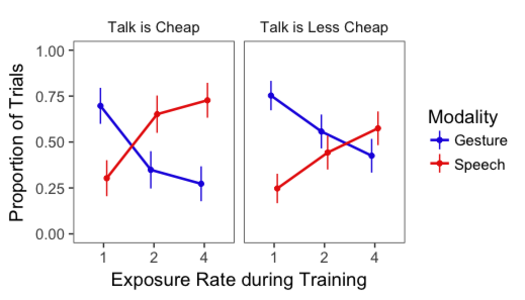
\includegraphics{figs/image1-1} 

}

\caption[Plot of modality choice as a function of exposure, split by utility condition]{Plot of modality choice as a function of exposure, split by utility condition.}\label{fig:image1}
\end{figure}
\end{CodeChunk}

\section{Experiment 2}\label{experiment-2}

Thus far, we have focused on relatively straightforward scenarios to
demonstrate that a pressure to communicate successfully in the moment
can lead speakers to trade-off between gesture and speech sensibly.
However, critical to these repeated interactions is the ability to learn
about an interlocutor and potentially influence their learning. In
Experiment 2, participants were told about a third type of message using
both gesture and speech within a single trial to effectively teach the
listener an object-label mapping. This strategy necessitates making
inferences about the listener's knowledge state, so we also manipulated
listener knowledge in Experiment 2.

\subsection{Participants, Materials,
Methods}\label{participants-materials-methods-1}

240 participants were recruited though Amazon Mechanical Turk and
received a small payment for their participation. 40 participants were
run in each of 6 different conditions, crossing our utility manipulation
(the same described in Experiment 1) and our partner knowledge
manipulation (where we told speakers that the listener had seen the
object-label pairs zero times, half as many times as the speaker, or
twice as many times as the speaker). 39 participants were excluded from
the final analysis for failing to respond correctly to the manipulation
check, producing pseudo-English labels, or producing nonsense labels
(e.g., ``xhlfjh'').

In order to produce teaching behavior, speakers had to pay the cost of
producing both cues, yielding 30 points in either condition of our
explicit points framework. Our communicative game was designed to reward
in-the-moment communication, and teaching required the speaker paying a
cost upfront. However, rational communicators may understand that if one
is accounting for future trials, paying the cost upfront to teach the
listener allows a speaker to use a less costly message strategy on
subsequent trials.

Incorporating teaching means that our speaker must now reason about
their interlocutor's knowledge state more explicitly, in order to make
rational decisions about what to teach and when. To address this added
dimension, we also manipulated participants' expectations about their
partner's knowledge. Prior to beginning the game, participants were told
that there partner had no experience with the lexicon, had half the
experience of the speaker, or had twice the experience of the speaker.

Listeners starting knowledge state were also initialized accordingly.
Listeners with no exposure were given no knowledge of the lexicon to
start. Listeners with half the exposure of the speaker began with
knowledge of three object-label pairs (2 high frequency, 1 mid
frequency), based the average retention rates found previously. Lastly,
the listener with twice as much exposure as the speaker began with
perfect knowledge of the lexicon, again based on the average retention
rates. Through gesture-speech co-occurrence, the speaker could
effectively teach the listener a novel mapping. Listeners could learn a
novel mapping from one teaching event in this game and integrate it into
their set of candidate words when evaluating the LD of subsequent
labels.

\subsection{Results}\label{results-1}

In line with our hypotheses, Experiment 2 mirrored the effects found in
Experiment 1 and demonstrated that teaching is also sensitive to these
same factors. A mixed effects logistic regression predicting whether or
not teaching occurred on a given trial revealed that teaching rates
across conditions depend on all of the same factors that predict speech
and gesture. There was a significant effect of initial exposure to the
mapping on the rates of teaching, such that more exposures to a word
predicted higher rates of teaching behavior (B = 0.09, p \textless{}
0.05). There was also a significant effect of the utility manipulation
such that being in the Talk is Cheap condition predicted higher rates of
teaching than being in the Talk is Less Cheap condition (B = 1.07, p =
0.01), a rational response considering teaching allows one to use a less
costly strategy in the future and that strategy is especially superior
in the Talk is Cheap condition.

As a predictor in our model, we also included whether this was an
objects first, second, or third appearance in the game. The expected
utility of teaching on a given trial should decrease as there are fewer
subsequent trials for that object, thus we predicted that teaching rates
would drop dramatically. Indeed, this is consistent with the results
from our model; compared with the first appearance of an object,
speakers were significantly less likely to teach on the subsequent
appearances (B = -1.02, p \textless{} 0.001).

\begin{CodeChunk}
\begin{figure}[H]

{\centering 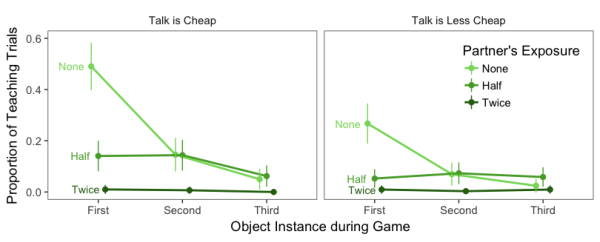
\includegraphics{figs/image3-1} 

}

\caption[Proportion of teaching behavior as a function of whether it was the first, second, or third appearance of a given target, split by partner's level of exposure]{Proportion of teaching behavior as a function of whether it was the first, second, or third appearance of a given target, split by partner's level of exposure.}\label{fig:image3}
\end{figure}
\end{CodeChunk}

Interestingly, as we expected, there was a significant effect of our
manipulation of listener knowledge. Speakers were significantly less
likely to teach the more exposure their partner had to the lexicon (B =
-1.45, p \textless{} 0.01). The data from Experiment 2 provide a proof
of concept that teaching behaviors can emerge from a pressure to
communicate successfully in the moment, especially when there is an
asymmetry in knowledge such that the speaker is interacting with a less
knowledgeable listener.

\section{Experiment 3}\label{experiment-3}

As a replication and extension of experiments 1 and 2, we sought to
embed the relative utilities of the communicative strategies in the
gameplay more implicitly. In experiment 3, we used the same procedure
described above; however, a timer controlled the number of points that
were earned on each trial of gameplay (Figure \ref{fig:imp_screenshot}).
Rather than impose an explicit point system as in experiments 1 and 2,
we set the relative utilities of communication strategies by
manipulating the speed with which participants could respond.

\begin{CodeChunk}
\begin{figure}[H]

{\centering 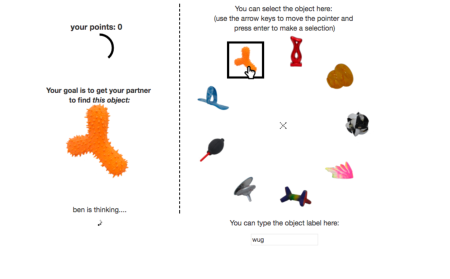
\includegraphics{figs/imp_screenshot-1} 

}

\caption[Screenshot of speaker view during gameplay in the Experiment 3 version]{Screenshot of speaker view during gameplay in the Experiment 3 version.}\label{fig:imp_screenshot}
\end{figure}
\end{CodeChunk}

\subsection{Participants, Materials,
Methods}\label{participants-materials-methods-2}

405 participants were recruited though Amazon Mechanical Turk and
received a small payment for their participation. Roughly 45
participants were run in each of 9 conditions, again crossing partner
knowledge (none, half as much, twice as much) with our utility
manipulation (pointing is normal, slow, or slowest). The responses from
128 participants were excluded for failing to meet our manipulation
check, using pseudo-English labels, or using non-sense labels.

Experiment 3 utilized the same training and pretest procedures, but
gameplay differed in a number of ways. During the game, the nine novel
objects were arranged in a circle around a cartoon pointer (see Figure
\ref{fig:imp_screenshot}). To manipulate the relative speeds of
gesturing and labeling, we required speakers to move the small pointer
with the arrow keys on their keyboards in order to select an object with
gesture. With this method we could directly manipulate the speed of the
pointer while holding the arrow keys to effectively set the maximum
possible utility of using gesture.

If the listener correctly identified the target object, speakers
received points determined by the amount of time remaining on the timer.
For successful communications, speakers always received a minimum of 10
points, regardless of the time elapsed. Based on pilot response times,
the timer was set to 6.5 seconds and points were scaled to match
experiments 1 and 2. Participants were randomly assigned into one of
three conditions, where the pointer was set to either a normal, slow, or
slowest setting.

This framework allowed us to implement the point system as an implicit
extension of gameplay and resulted in each participant having unique
gesture-speech utilities, based on the speed of their responses across
the two methods.

\subsection{Results}\label{results-2}

In Experiment 3, we see gesture and speech trading off in the same
patterns as Experiments 1 and 2. A mixed effects logistic regression
showed that the more exposure to a given object during training, the
more likely speakers were to label that object during the game (B =
0.53, p \textless{} 0.01).

\begin{CodeChunk}
\begin{figure}[H]

{\centering 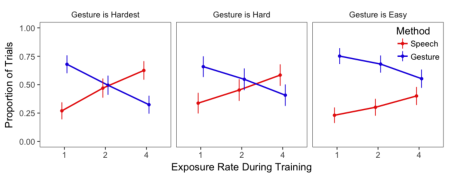
\includegraphics{figs/imp_speech_gesture-1} 

}

\caption[Speakers' communicative method choice as a function of exposure and the utility manipulation]{Speakers' communicative method choice as a function of exposure and the utility manipulation. These data are taken only from the condition where listeners had more exposure to the lexicon than speakers, as the speech-gesture trade-off is most easily interpreted here. Rates of teaching not show.}\label{fig:imp_speech_gesture}
\end{figure}
\end{CodeChunk}

Critically, there was a main effect of our utility manipulation, such
that speakers the more difficult it was to gesture, the more likely
participants were to rely on speech (B = 0.09, p \textless{} 0.01).
Figure \ref{fig:imp_speech_gesture} illustrates this pattern in the
condition where the listener has more exposure than the speaker, as
there was minimal teaching in that condition and thus the speech-gesture
trade-off is most interpretable. In the absence of an explicit framework
for assigning utilities based on method, speakers continue to adapt
their communicative choices taking into account the expected utility of
possible strategies.

Rates of teaching behavior also held a similar pattern shown in
Experiment 2. We fit a mixed effects logistic regression to predict
whether or not participants taught on a given trial, using the same
predictors from Experiment 2. The number of remaining trials for a given
object persisted as a significant predictor, again finding that later
appearances of an object are less likely to evoke teaching (B = -0.94, p
\textless{} 0.001). The role of listener knowledge also remained
similar, such that the more exposure the listener had to the lexicon,
the less likely speakers were to teach (B = -1.15, p \textless{} 0.001).
Despite these similarities, the effects of our utility manipulation and
the initial exposure rate were not significant on the rates of teaching
(B = -0.03, p \textgreater{} 0.05 and B = 0.10, p \textgreater{} 0.05,
respectively). This is possibly due to the unexpected noise in the data
in the Gesture is Hardest, Partner has twice the exposure condition (see
Figure \ref{fig:imp_speech_gesture}). Nevertheless, these results
corroborate our early findings, demonstrating that teaching behavior
emerges in both a paradigm with an explicit points system (Experiment 2)
and an implicit points system (Experiment 3), despite the initial cost.

\begin{CodeChunk}
\begin{figure}[H]

{\centering 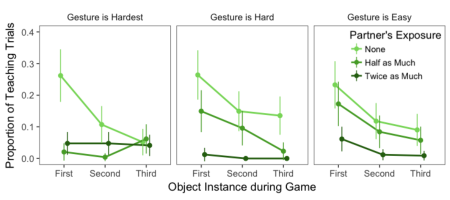
\includegraphics{figs/imp_teach-1} 

}

\caption[Rates of teaching across the partner exposure manipulation and appearances taken from gameplay in Experiment 3]{Rates of teaching across the partner exposure manipulation and appearances taken from gameplay in Experiment 3.}\label{fig:imp_teach}
\end{figure}
\end{CodeChunk}

\section{Model: Iterated Communication as Rational
Planning}\label{model-iterated-communication-as-rational-planning}

The results from these experiments are qualitatively consistent with a
model in which participants make their communicative choices to maximize
their expected utility from the reference game. We next formalize this
model to determine if these results are predicted quantitatively as
well.

\newcommand{\E}[1]{\mathbb{E}\left[ #1 \right]}

In a one-shot reference game maximizing expected utility is simply
choosing the action (\(a\)) that has the highest expected utility
\((\E{U})\). The expected utility depends both on the action itself, and
on the state of the two partners (\(s\)): For pointing, this expected
utility is independent of referent, defined entirely by our experimental
manipulation. In contrast, for speech, the utility varies with the
probability of partners sharing a common label for the referent.
Following other models in the Rational Speech Act framework, we use the
Luce Choice Axiom, in which each choice is taken in probability
proportional to its exponentiated utility (Frank \& Goodman, 2012). This
choice rule has a single parameter \(\alpha\) that controls the noise in
this choice--as \(\alpha\) approaches 0, choice is random and as
\(\alpha\) approaches infinity choice is optimal:

\[ 
C\left(a;s\right) \propto e^{\alpha \E{U \left(s,a\right))}}
\]

To use this rule, agents have to estimate how likely they are to share a
common label (\(s\)). In our simulation, we assume for simplicity that
people have an accurate representation of their own knowledge. We thus
set each simulated participant's knowledge to the explicit recall
judgment made by a real participant in our experiments. To estimate
their partner's knowledge, participants can reason about their own
learning. Again for simplicity we model learning as a simple Bernoulli
process: Each exposure to novel label is like a flipping a coin with
weight \(p\), if it comes up heads, the label is learned. Having
observed their own learning outcomes, agents can infer their own
learning rate by determining the weight \(p'\) under which their
observed learning is most likely. Assuming that their partner would have
learned at the same rate, participants can then generate a probability
with which their partner would have learned each label by estimating the
probability that at least one of its \(n\) came up heads given learning
rate \(p'\): \(P\left(s^{+}\right)=1-p'\left( 1-p' \right)^{n}\).

In an iterated game, however, because actions taken on the current trial
can influence the state (\(s\)) on future trials, the optimal action to
take is not the one that optimizes the single trial's rewards, but
rather the one that optimizes the expected rewards that will accumulate
over all future trials (Kaelbling, Littman, \& Cassandra, 1998).

For the results reported here, we set \(\alpha = 2\) based on
hand-tuning, but other values produce similar results.

\begin{itemize}
\tightlist
\item
  Discounting parameter
\item
  Leploss parameter
\end{itemize}

We implemented a two-agent model of speaker and listener behavior in
this game based on partially observable Markov decision processes. The
speaker is given a target referent each trial and must signal to the
listener which object to select. Speakers send messages to the listener
by speaking, a low cost cue that relies on the listener's knowledge, or
by pointing, a higher cost cue that is unambiguous.

The speaker estimates the listener's knowledge. First, the speaker uses
Markov chain Monte Carlo to infer their own learning rate based on how
well they were able to learn a novel lexicon after N exposures. Then,
given the listener's degree of exposure, the speaker can use their own
learning rate to infer the probability that the listener would know any
given object-label mapping. Across trials, the speaker gains further
information about the listener through their selections, allowing them
to update their beliefs about the listener's knowledge state.

The model specifies the relative costs for each communicative modality.
On each trial, the speaker estimates the expected utility of each
modality by accounting for these costs, their own knowledge of the
object's label, and the probability that the listener knows the object's
label. The speaker then uses Luce's choice axiom to select a
communicative modality based on the expected utilities.

When estimating expected utility, the model sums the expected utility of
a given trial and any remaining trials for that particular object. This
allows the speaker to engage in planning by accounting for the way a
given message may induce knowledge changes and thus affect subsequent
expected utilities. Utilities were scaled using an exponential
discounter as a function of delay to give greater weight to immediate
rewards than subsequent rewards.

Crucially, speakers can also combine both communication cues, paying the
upfront cost of both, to produce a message that is both unambiguous and
informative. In this way, speakers are able to teach their partners
object-label mappings. A speaker that plans may thus infer that teaching
the listener, especially if there is an asymmetry in their knowledge
states, may have a high expected utility after accounting for remaining
trials where the speaker could use a less costly cue (i.e.~speech).
After producing both cues, the speaker also updates their own beliefs
about the partner's knowledge state to reflect this exposure.

\begin{CodeChunk}
\begin{figure}[H]

{\centering 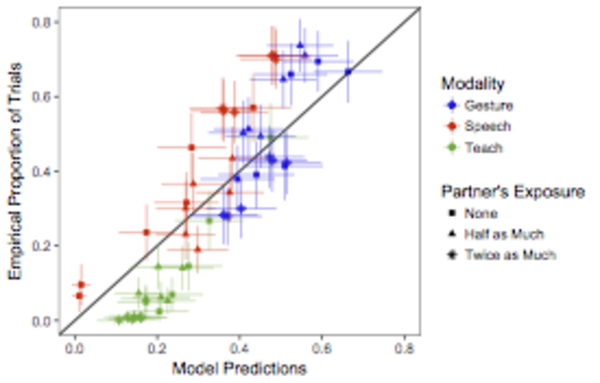
\includegraphics{figs/image4-1} 

}

\caption[Plot of the fit between model predictions and empirical data]{Plot of the fit between model predictions and empirical data.}\label{fig:image4}
\end{figure}
\end{CodeChunk}

\section{Discussion}\label{discussion}

\section{Acknowledgements}\label{acknowledgements}

We are grateful to Elliot Lipnowski for thoughtful feedback on the
model. This research was funded by a James S. McDonnell Foundation
Scholar Award to DY.

\section{References}\label{references}

\setlength{\parindent}{-0.1in} \setlength{\leftskip}{0.125in} \noindent

\hypertarget{refs}{}
\hypertarget{ref-bloom2000}{}
Bloom, P. (2000). \emph{How children learn the meanings of words}. MIT
press: Cambridge, MA.

\hypertarget{ref-blythe2010}{}
Blythe, R. A., Smith, K., \& Smith, A. D. M. (2010). Learning times for
large lexicons through cross-situational learning. \emph{Cognitive
Science}, \emph{34}, 620--642.

\hypertarget{ref-brown1977}{}
Brown, R. (1977). Introduction. In C. E. Snow \& C. A. Ferguson (Eds.),
\emph{Talking to children: Language input and interaction}. Cambridge,
MA.: MIT Press.

\hypertarget{ref-eaves-jr2016}{}
Eaves Jr, B. S., Feldman, N. H., Griffiths, T. L., \& Shafto, P. (2016).
Infant-directed speech is consistent with teaching. \emph{Psychological
Review}, \emph{123}(6), 758.

\hypertarget{ref-frank2012}{}
Frank, M. C., \& Goodman, N. D. (2012). Predicting Pragmatic Reasoning
in Language Games. \emph{Science}, \emph{336}(6084), 998--998.

\hypertarget{ref-kaelbling1998}{}
Kaelbling, L. P., Littman, M. L., \& Cassandra, A. R. (1998). Planning
and acting in partially observable stochastic domains. \emph{Artificial
Intelligence}, \emph{101}, 99--134.

\hypertarget{ref-mcmurray2013}{}
McMurray, B., Kovack-Lesh, K. A., Goodwin, D., \& McEchron, W. (2013).
Infant directed speech and the development of speech perception:
Enhancing development or an unintended consequence? \emph{Cognition},
\emph{129}(2), 362--378.

\hypertarget{ref-newport1990}{}
Newport, E. L. (1990). Maturational Constraints on Language Learning.
\emph{Cognitive Science}, \emph{14}(1), 11--28.

\hypertarget{ref-newport1977}{}
Newport, E. L., Gleitman, H., \& Gleitman, L. R. (1977). Mother, I'd
rather do it myself: Some effects and non-effects of maternal speech
style. In C. A. Ferguson (Ed.), \emph{Talking to children language input
and interaction} (pp. 109--149). Cambridge University Press.

\hypertarget{ref-saffran2003}{}
Saffran, J. R., \& 2003. (2003). Statistical language learning:
Mechanisms and constraints. \emph{Current Directions in Psychological
Science}, \emph{12}(4), 110--114.

\hypertarget{ref-smith2008}{}
Smith, L. B., \& Yu, C. (2008). Infants rapidly learn word-referent
mappings via cross-situational statistics. \emph{Cognition}, \emph{106},
1558--1568.

\hypertarget{ref-smith2013}{}
Smith, L. B., \& Yu, C. (2013). Visual attention is not enough:
Individual differences in statistical word-referent learning in infants.
\emph{Language Learning and \ldots{}}, \emph{9}, 25--49.

\hypertarget{ref-vlach2013}{}
Vlach, H. A., \& Johnson, S. P. (2013). Memory constraints on infants’
cross-situational statistical learning. \emph{Cognition}, \emph{127}(3),
375--382.

\hypertarget{ref-vogt2012}{}
Vogt, P. (2012). Exploring the robustness of cross-situational learning
under zipfian distributions. \emph{Cognitive Science}, \emph{36}(4),
726--739.

\hypertarget{ref-yurovsky2017}{}
Yurovsky, D. (2017). A communicative approach to early word learning.
\emph{New Ideas in Psychology}, 1--7.

\end{document}
